\documentclass{article}
\usepackage{dsfont}
\usepackage{graphicx} % Required for inserting images
\usepackage{subcaption} % for mulitple images
\usepackage[fontsize=12pt]{fontsize} % font size
\usepackage{setspace}
\usepackage[margin=1.5cm, headheight=15pt]{geometry} % layout of the document
%\usepackage{hyperref} % Hyperlink
\usepackage{amsthm} % Writing theorem
\usepackage{amsmath} % Maths notations 
\usepackage{amssymb} % For sets character
\usepackage{enumitem} % For charctere in enumeration
% \usepackage{unicode-math}
\usepackage{mathtools}
\usepackage{booktabs}

\newtheorem{definition}{Definition}
\newtheorem{proposition}{Proposition}
\newtheorem{theorem}{Theorem}

\usepackage[colorlinks=true,
            linkcolor=blue,
            citecolor=blue,
            urlcolor=blue]{hyperref}

%\hypersetup{pdfborder=0 0 0}
\usepackage{cleveref}
\setstretch{1.5} % space between lines
\setlength{\parindent}{0pt}
\usepackage{listings}
\usepackage{color}

\definecolor{dkgreen}{rgb}{0,0.6,0}
\definecolor{gray}{rgb}{0.5,0.5,0.5}
\definecolor{mauve}{rgb}{0.58,0,0.82}
\lstset{frame=tb,
  language=C,
  aboveskip=3mm,
  belowskip=3mm,
  showstringspaces=false,
  columns=flexible,
  basicstyle={\small\ttfamily},
  numbers=none,
  numberstyle=\tiny\color{gray},
  keywordstyle=\color{blue},
  commentstyle=\color{dkgreen},
  stringstyle=\color{mauve},
  breaklines=true,
  breakatwhitespace=true,
  tabsize=3
}

\usepackage{biblatex}
\addbibresource{reference.bib}


\title{LIDAR and autonomous robot navigation algorithm implementation}

\author{
Jessica Xu, 261163415
}

\date{Winter 2026}

\begin{document}

\maketitle

\begin{figure}[ht!]
    \centering
    
\includegraphics[width=0.5\linewidth]{Mcgill_university_coa.png}
\end{figure}

\begin{center}
    Project presented to Professor Joseph Vybihal
\end{center}

\begin{center}
    COMP 400
\end{center}

\newpage
\tableofcontents

\newpage
\section{Introduction}
In robotics, the physical build is often viewed as the most complex procedure , but the true complexity lies in the digital brain that navigates the physical world. The ability to navigate an unmapped environment is the main core of autonomous robotics. In many real-world-scenarios, robots can't always rely on pre-loaded maps or GPS data. A couple examples include search-and-rescue mission and automated warehousing. These environments are often dynamic and unpredictable. \\

For the $R1D4$ project, my goal is to get the robot to the door in a randomly placed indoor classroom. Therefore, no initial map is given to the robot. To be able to connect the gap between raw data and actionable data, and with the access to a pulse Lidar and a webcam, we have decided to add a sensor system. The motivation behind the $R1D4$ project is to develop a robust simultaneous localization and mapping that does not only move through space, but does it intelligently. \\

Since the first step of this project is to make the robot recognize the door, colored image will be used as a feature on the webcam to feed the input of a trained model, then I will use the Lidar for the mapping algorithm as it is computationally lighter, more efficient and higher spacial accurate, so I can then use to map the path. The final path mapping system is made by smartly creating nodes it can go to between obstacles that it sees called dynamic graph generation, to have the most optimatel path.

\section{Background}

To understand the navigation and recognition logic of the $R1D4$ project, it is necessary to establish some definitions. First, how does the Lidar work? The Lidar system operates on a Time-of-Flight (ToF) principle which consists of four cour subsystems: a laser emission system, a scanning system, a laser reception system and a signal processing system \cite{IBM_LiDAR}. Therefore, the laser will emit a laser beam towards a target, then the laser reception system will receive the signal back, which will be able to characterize the surface it hit, including the distance. Originally, we wanted to use the depth camera, just like its name, allows us to capture the depth in the picture, but also gives a colored image output. \\

The main challenge of this project is solving a SLAM problem. SLAM involves an autonomous robot building a map of an unknown environment while simultaneously keeping track of its own location \cite{MathWorks_SLAM}. Since $R1D4$ starts without a floor plan, it must use the sensors to create a set of data points in space to calculate its trajectory. Although no single sensor is perfect, Lidar is highly accurate for distance but blind to color and texture. Originally, this is where the depth camera comes into play, by providing a coloured image and depth information, but can be sensitive to lighting and uses more processing power. By doing a sensor fusion, we could have fused these two sensors, with our approach of the camera identifying the target, while the Lidar provides obstacle avoidance data needed to reach it. \\

Then, for the main path finding algorithm, it will use dynamic graph generation. It involves the real-time creation and update of nodes representing the robot poses, with the edges representing spatial constraints, which will be modelled in an evolving environment \cite{cho2024open}. This allows the robot to adapt its path planning on the fly, as it receives sensor data, in my case, the Lidar points . \\ 

I will also train datasets and use YOLO for the recognition of the door in an image and create a path finding algorithm. YOLO is a popular, high-speed and accurate real-time object detection algorithm. YOLO (You Only Look Once) has evolved from a purely convolutional architecture into a model that incorporates transformers. The image is treated as a sequences of patches which allows the model to use self-attention mechanism to relate distance objects to one another \cite{GeeksforGeeks_YOLO}. It is assumed the reader knows the basics of machine leraning. 

\section{Getting the camera and lidar to work}

The model of the $3D$ Depth camera that we would have used is a Nuwa-HP60C 3D depth camera. It uses a binocular structured light, which is designed for robotics and navigation. The model offers a $0.2m-4m$ depth range, a $73.8^\circ$ field of view and $640\times480$@$30$fps depth output \cite{RobotShop_Yahboom_Nuwa}. 
I had a positive start with the Lidar, but unfortunately for the depth camera, we learned that we can't be using ROS to operate it. No documentation could be found online, therefore we have decided to use an alternative way of operating the detection of door by using a standard webcam. \\

Now for the Lidar, at first, the SDK I found was not working with this lidar so I had to parse the packs myself. Fortunately, it was able to connect to a laptop via the USB-A cable, so I was able to work on it directly with python code. The lidar constantly spams packets which each contains 12 points each. A point consist of (angle, distance, intensity). The angle is the angle of the point from the starting point of the lidar, the distance is the distance from the lidar and the intensity is the intensity of the light reflected back to the lidar. First, it's important to check the integrity of the data. Then, the most important part is to be able to parse the data and make it useful. By creating the STL19P class, it was possible to read the packet and parse them, to then be able to display the result.\\

The lidar can detect and replace the depth ability of the camera, but it can't check that in an entire frame (only $360^\circ$ at a specific height). This was is an issue but in the time-span, the webcam is an efficient and simple replacement. 



\section{Planning for the algorithm for the mapping and path planning of the robot}

Before even starting to program, some simple yet crucial assumptions needs to be established. First, it is assumed that the surface the robot navigates one is a flat 2D surface. Second, the door remains open and is a narrow rectangle that sits between two parallel wall segment. Third, the map is not given to the robot, and the environment changes everytime. Then, the obstacles should be at least the height of the camera/Lidar. Lastly, it is assumed the obstacles will remain static. \\

Now, to figure out how the robot can recognize where the door is in a indoor room, I had the naive idea of not doing anything too complicated, that is create an algorithm that recognizes the door by using step detection. This is done by taking advantages of the gap between the left and right frame of the door. If there is a sudden increase in depth between them, then the door should be located there. Therefore, using the depth camera, it would be possible to calculate the euclidean distance between two corners. Here is how it would look like pseudocode wise: \\\\
Algorithm to identify the door (step detection): \\
- Left frame (left side of the door): Sudden increase in depth. \\
- Gap: Empty space between the frames \\
- Right frame (right side of the door): Sudden decrease in depth. \\
- Calculate the euclidean distance between two corners $(x_1, y_1)$ and $(x_2, y_2)$. If the distance fits a doorframe distance, then most likely found a door. \\\\
This algorithm is simple, but also adds more assumptions on the classroom's structure, that is, gaps may exists between the walls, yet the door is not located there. It will most likely also make the overall path finding algorithm longer, since the robot has to go around the classroom. I therefore decided to use machine learning, which will train a model instead to recognize where the door is in a picture. \\\\
Then, for the navigation algorithm, I had many plans. The simplest one being hugging the wall, also known as Frontier exploration \cite{Liu_ScientificReports_2025}. The robot will go around the classroom, while being at a certain distance from the wall, and once it sees the door, it will definitively being able to go through it since a door is mounted to a wall. Overall, this is obviously not efficient therefore the next plan is to use RRT. \\


\subsection{Mapping (Probabilistic road map for path planning)}
Before starting with the algorithm, some definitions need to be stated. What is exactly Path Planning? Path planning is a computational problem that lets an autonomous mobile robot find the best or the most optimal path between two points \cite{Khokhar_PRM_2021}.
The goal is to find the shortest path between the two points, taking in consideration obstacles in its path. \\

The probabilistic Roadmap planning (PRM) is therefore used to determine the shortest path between two points, while avoiding collisions with obstacles. Since I will be using graphs, I will refer to these points as nodes (a.k.a. vertices). PRM consists of two phases: a construction phase and a query phase. In the construction phase, a network graph of possible paths based on free and occupied spaces is created. Here are the steps to create such network graph: 
\begin{enumerate}
    \item A random samples from the configuration space of the robot is created, therefore a random node is generated in the configuration space.
    \item The system checks if the node lies in a free space or not. If the node is in a free space, it is will be added to the graph. 
    \item This new node will connect to the closest nodes through a straight line. 
    \item The system checks if the connection between the two nodes lies in a free space or not (if there is an obstacle or not). If it does, the connection is added to the graph between the two nodes.
\end{enumerate}

Typically, it connects to $k$ nearest neighbors. In the query phase, the start and goal configurations are connected to the graph. Therefore, at this stage, you can create a complete graph \cite{Khokhar_PRM_2021}. To obtain the shortest path, Dijkstra's algorithm will be used. This all sounds nice on paper, but won't work since the environment is not static. \\


\subsection{Rapidly exploring random tree (RRT)}

Since environment is not static (the map can change everytime), it's more efficient to use RRT since it's best with single-query goals. \\

Now, the use of RRT is actually pretty straight forward. You start by generating a set of random points, which will be connected to the closest vertices. That is, every time new vertex is created, it's important to check if the vertex is not part of the obstacle, including the edge that connects the two vertices or the neighborhood vertices. RRT allows us to create the mapping and find the shortest path \cite{Chinenov_RRT_2019}. \\

My teammate already started working on a RRT algorithm which is based of a given map. He was able to successfully create a visual environment, given a map. The whole skeleton was already made, but a lot of changes had to be done, the most important one being that the robot moves every time it finds a new node, since no map will be given to the robot. I first changed the data structure, then changed how the robot moves, in every iteration. The implementation is now more accurate to a tree and cleaner, with a root, a tuple of $(x, y)$ coordinates for each node, and a tuple of indices for the edges, connecting the parent and child nodes. To start of, a running test was done on a simulated environment without incorporating the bias. The number of iterations were much higher than if it included the bias. The bias is really useful when the position of the goal is known, in my case, the door. The results do change since nodes are randomly generated, but the bias was necessary and improved the number of steps it took for the robot to get to the door. The issue with this algorithm is it's actually not useful at all for the real world implementation on the robot, since it will uses the assumption that the map is given to the robot.\\

After the suggestion I got from professor Joseph Vybihal, it was decided to completely scratch the idea of using RRT, and instead implement my own path finding algorithm, which overall relies on finding an efficient point where the robot can see at that time and go there, called dynamic graph generation using adaptive point clustering. 

\section{The algorithms I implemented}

\subsection{Model that can recognize a door}
Instead of selecting a specific length for the door by using the depth array (as described in the idea above), it is better to train a model that can recognize what is a door in an image. First, I had to find a dataset to train the door detection model with. I first tried with a dataset composed of $400$ inside door gpg images and labels, found on kaggle \cite{sayedmohamed_2023}. Since for this project, we are assuming the robot is indoor, I changed the dataset with a set of $581$ images. The labels are composed of a tuple of $5$ values: the class, the localization of the point on an image, given by $x$, localization of the point on an image, given by $y$, width and height. I will use YOLO (you only look at it once) model instead of the conventional way of building a CNN, more precisely, it will be a fine-tune YOLO, that is, on top of an already trained model done by Ultralytics \cite{Jocher_Ultralytics_YOLO_2023}, I will add the specification to recognize what is an inside door. \\

First, I had to filter the dataset, since it was not solely composed of doors. The original dataset had $1213$ images \cite{Arduengo_2021}, but I had to remove two third of the dataset as it had other images that were not indoor doors. To avoid overfitting and increase the generalization, data augmentation was used on the pictures. 


\subsection{My own path finding algorithm}

First, my datastructure of the path finding algorithm is a tree, where each nodes has: a position coordinate $x, y$, if it's visited (bool) and if it's an intermediate created node (bool). Every time the robot goes to that node, it is marked as visited. \\

Now, I have to do my own path finding algorithm which relies on the logic of what the robot sees. The lidar will return a bunch of LidarPoints which features the obstacles it sees. First, I decided to create many list of cluster points (points that are close to each other). Here are the requirements for the LidarPoints to be in the same clusters: points next to each other angle wise and the points need to be close enough with respect to a dynamic threshold on their distance relative to the lidar. This function assumes that the points are sorted by angles. Here is the pseudo code:\\
\begin{lstlisting}[language=Python, caption=Adaptive Lidar Point Clustering Pseudocode]
# --- Initialization ---
IF list of points is empty:
    RETURN an empty list

INITIALIZE ls_cluster as a list containing [first point]

# --- Step 1: Sequential Grouping ---
FOR EACH current_point in ls_point (from second point):
    last_point = last point added to the most recent cluster
    
    # Calculate smallest angular difference (360 wrap-around)
    diff_angle = abs(current_point.angle - last_point.angle)
    diff_angle = MIN(diff_angle, 360.0 - diff_angle)
    
    # Calculate expected spatial gap (Arc Length)
    min_dist = MIN(current_point.distance, last_point.distance)
    expected_gap = min_dist * RADIANS(diff_angle)
    
    # Compute the adaptive threshold
    adaptive_delta = (expected_gap * margin_factor) + noise_margin
    
    # Check if points are physically close enough
    IF EuclideanDistance(current_point, last_point) < adaptive_delta:
        Add current_point to the current (last) cluster
    ELSE:
        Start a NEW cluster with current_point
        
# --- Step 2: 360-Degree Wrap-around Check ---
IF length(ls_cluster) > 1:
    first_pt = first point of the first cluster
    last_pt = last point of the very last cluster
    
    diff_angle = MIN(abs(first_pt.angle - last_pt.angle), 360.0 - abs(...))
    expected_gap = MIN(first_pt.dist, last_pt.dist) * RADIANS(diff_angle)
    adaptive_delta = (expected_gap * margin_factor) + noise_margin
    
    IF EuclideanDistance(first_pt, last_pt) < adaptive_delta:
        Merge the last cluster into the start of the first cluster
        Remove the last cluster from the list
        
# --- Step 3: Filtering by Size ---
FOR EACH cluster in ls_cluster:
    IF length(cluster) < min_cluster_size:
        Remove this cluster from the results
        
RETURN ls_cluster
\end{lstlisting}

Then I had to find the extremities of the cluster it sees to set the path algorithm. To find the extremities, it was done by choosing the points with the smallest and biggest angle in the cluster points, except if the cluster spans the $0^\circ$ and $360^\circ$. In that case, all the angles were shifted until it does not overlap these two angles. The pseudo code is given by:
\begin{lstlisting}[language=Python, caption=Finding Cluster Extremities with Wrap-around Handling]
# --- Step 1: Extract Angles ---
INITIALIZE ls_angle as an empty list

FOR EACH point in cluster:
    Add point.angle to ls_angle
    
SET done to TRUE

# --- Step 2: Check for 0/360 Degree Overlap ---
FOR EACH angle in ls_angle:
    IF angle > 359 OR angle < 1:
        # The cluster is sitting on the boundary line
        SET done to FALSE
        BREAK loop
        
# --- Step 3: Shift Angles (Virtual Rotation) ---
# Rotates coordinates until no points sit on the 0-degree boundary
WHILE done is FALSE:
    FOR EACH index i in ls_angle:
        # Increment angle by 1 degree and wrap at 360
        ls_angle[i] = (ls_angle[i] + 1) MODULO 360
        
    SET done to TRUE
    
    # Verify if the new rotation is clear of the boundary
    FOR EACH angle in ls_angle:
        IF angle > 359 OR angle < 1:
            SET done to FALSE
            # Continue rotating...
            
# --- Step 4: Identify Extremes ---
# In the shifted view, min/max values are the true cluster edges
index_min = Index of the SMALLEST value in ls_angle
index_max = Index of the LARGEST value in ls_angle

RETURN cluster[index_min] and cluster[index_max]
\end{lstlisting}

Now, the task is to find the list of nodes the robot can go to potentially (not necessarily reachable). First, the list of clusters are sorted according to the angle (small to big). This comes from my assumption above. The new points will be generated between two clusters, more precisely, between the extremities of each cluster. This is visually explained using figure $1$. After generating the points, the robot chooses randomly the point it will go to.\\

This is where one of the many challenges lies. The robot can't directly go to the green dots in figure $2$, since it will go into the obstacle, therefore I had a couple ideas, such as doing $90$ degree turns in blue dots featured in figure $2$. The robot would go to the yellow point before getting to the green node. This works for some points but the robot has the chance of getting stuck in the corners, or the intermediate point could go in collision with an obstacle. \\

\begin{figure}
    \centering
    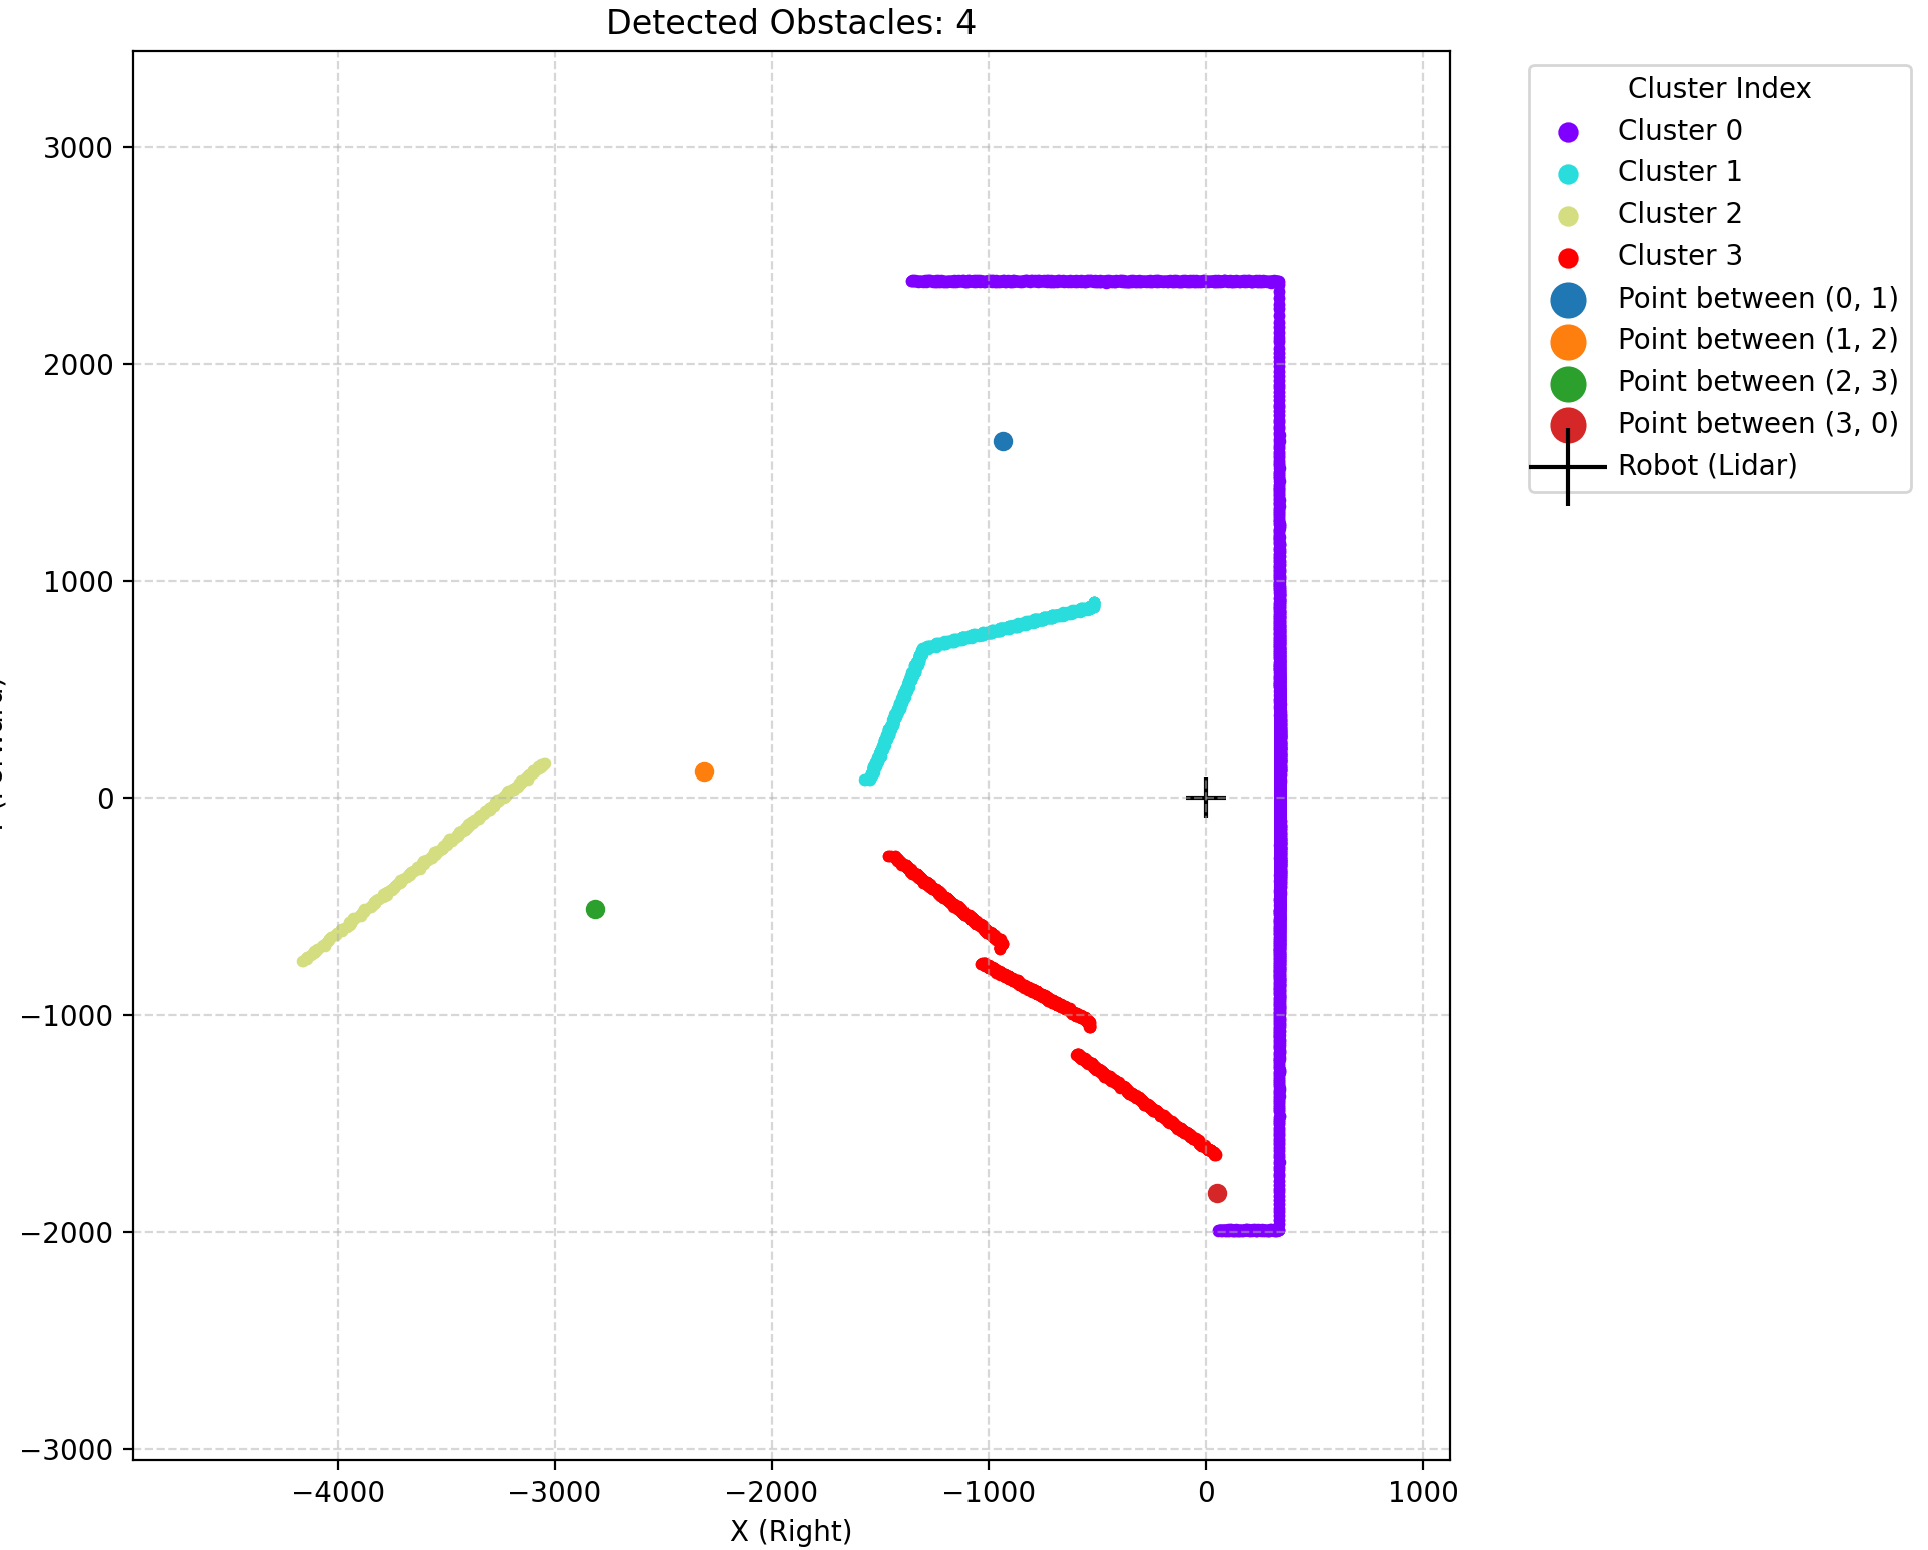
\includegraphics[width=0.5\linewidth]{points.png}
    \caption{All the different cluster point lists are in different colors, and the points you see are the possible spot the robot can go to}
    \label{fig:placeholder}
\end{figure}
\begin{figure}
    \centering
    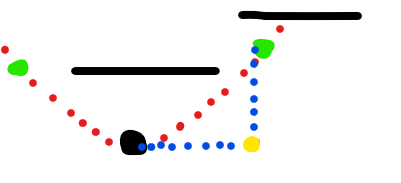
\includegraphics[width=0.5\linewidth]{path_planning.png}
    \caption{path planning using 90$^\circ$. The robot is the black dot and the green dots are the dots it should go to. The red doted lines represent what the robot sees at that instance. The black lines are the obstacles (cluster points)}
    \label{fig:placeholder}
\end{figure}
\begin{figure}
    \centering
    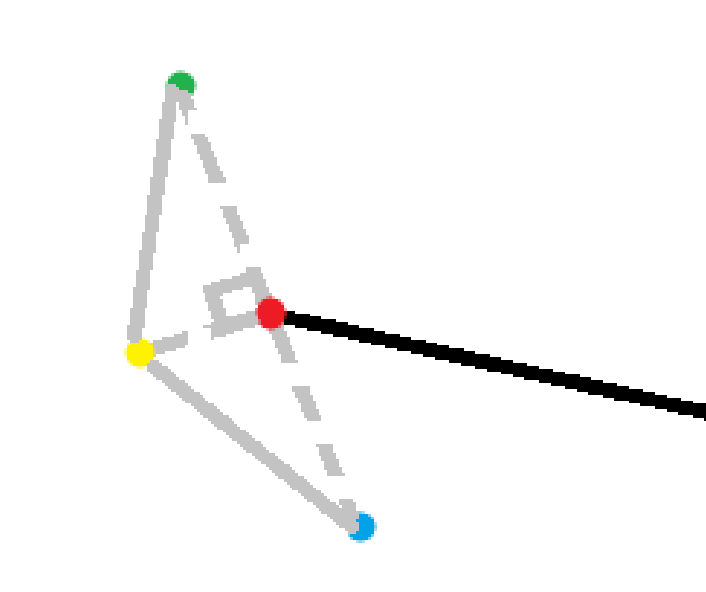
\includegraphics[width=0.5\linewidth]{intermediate_node.png}
    \caption{This figure shows how to generate the intermediate node correctly. The blue dot represents where the robot is, the green dot represents where the robot goes to. The red dot shows there is a collision pint there, and the yellow dot is the newly created intermediate node, following the gray dotted lines. The grey lines shows the new path the robot will take}
    \label{fig:placeholder}
\end{figure}
Instead of doing that, I decided to take advantage of the extreme points in the clusters, done in the function go-to. I added a safety margin so the robot does not bump into them. To illustrate this, let's say that the current position of the robot is at point $A$ and the point it wants to go is point $B$. The new intermediate points $P$ would therefore be the point that is perpendicular to the segment between $A$ and $B$, at the distance of safety margin. There are two possible coordinate $P$ that are the perpendicular points, so a neighbor of the extreme poin had to be chosent, which allows the robot to see if the obstacle is on the left or right of the segment between $A-B$. If it is on the left, then the point $P$ will be on the right of the obstacle, else the opposite. This is in recursion, that is, it will create intermediate until point $A$ can reach point $B$ safely. This process is illustrated in figure $3$. These points automatically have the status of being an intermediate point. Sometimes, points are possible to reach in a straight line (no need to add intermediate points), so I created a function that checks if the path is safe via a straight line. Here is the pseudo code of my function go-to: \\
\begin{lstlisting}[language=Python, caption=Recursive Obstacle Avoidance Path Planner]
# --- Step 1: Initialization ---
SET start_pos = coordinates of current robot position
SET end_pos = coordinates of target node
SET ls_nodes = [start_pos]
SET stack = [(start_pos, end_pos)]
SET iteration_count = 0

# --- Step 2: Recursive Path Verification ---
WHILE stack is NOT empty:
    IF iteration_count > 5: 
        RETURN NULL # Fail-safe limit reached
    
    (current_start, current_end) = stack.POP()
    iteration_count = iteration_count + 1

    # Check if segment hits an obstacle
    is_safe, (collision_pt, neighbor_pt) = is_path_safe(current_start, current_end, ls_cluster)

    IF NOT is_safe:
        # Check if cluster itself is too risky
        IF is_cluster_unsafe(collision_pt): 
            RETURN NULL
        
        # Calculate tangent angle to avoid collision
        angle_to_collision = ATAN2(coll_y - start_y, coll_x - start_x)
        
        IF collision_pt.angle < neighbor_pt.angle:
            avoidance_angle = angle_to_collision + 90 degrees
        ELSE:
            avoidance_angle = angle_to_collision - 90 degrees

        # Create waypoint outside collision zone
        offset_dist = robot_radius * (safety_margin + 0.2)
        new_waypoint = calculate_coords(collision_pt, avoidance_angle, offset_dist)

        # Split path into two segments and push back to stack
        stack.PUSH(new_waypoint, current_end)
        stack.PUSH(current_start, new_waypoint)

    ELSE:
        # Segment is clear! Add destination to path
        Append current_end to ls_nodes

# --- Step 3: Finalize and Graph Update ---
FOR EACH intermediate_point in ls_nodes:
    Create new node in global map
    Connect edge to previous node in path

# Calculate distances and angles for motor control
ls_pts_path = list of (x, y, distance, angle) for each segment
Update current_node = target_node_index

RETURN ls_pts_path
\end{lstlisting}
Now, once the robot is stuck in some sort of deadend, I made it go back to its step. Since my architecture is a tree, then the robot simply goes back to its parent node that has no visited children. This logic was implemented using a BFS algorithm. After it finds the node that is non visited, the lidar does another scan, find the new clusters, then reapply go-to. Here is the pseudo code:\\
\begin{lstlisting}[language=Python, caption=Robot Backtracking and Re-exploration Logic]
# --- Step 1: Backtrack to find a branch with unexplored nodes ---
INITIALIZE ls_path as an empty list
SET done to FALSE

WHILE done is FALSE:
    IF current_node is 0 (The Root):
        RAISE EXCEPTION "All nodes explored"

    # Identify the "Parent" path to move backwards
    SET ls_parents = [current_node, parent of current_node]
    
    # Climb up if current parent is an intermediate node
    WHILE last node in ls_parents is "Intermediate":
        Add parent of last node to ls_parents

    # Calculate movement to travel back up this path
    FOR EACH segment in ls_parents:
        dist = distance(current, parent)
        ang = angle(current, parent)
        Append (parent_x, parent_y, dist, ang) to ls_path

    # Update position and search for new targets
    current_node = last node in ls_parents
    target_node = BFS(current_node) # Nearest unvisited node

    IF target_node exists:
        SET done to TRUE

# --- Step 2: Navigate from Backtrack Point to New Target ---
SET temp = target_node
SET ls_nodes_to_target = []

# Trace path from new target back to current position
WHILE current_node is NOT temp:
    temp = parent of temp
    Add temp to ls_nodes_to_target

# Reverse movement to head toward the target
FOR EACH node in ls_nodes_to_target (from end to beginning):
    dist = distance to node
    ang = angle to node
    Append (node_x, node_y, dist, ang) to ls_path
    current_node = node

# --- Step 3: Final Approach ---
Refresh Lidar scan at new location
new_clusters = cluster(new_scan)

# Use avoidance logic for the final stretch
final_approach = go_to(target_node, new_clusters, safety_margin)
ls_path = ls_path + final_approach

RETURN ls_path
\end{lstlisting}

Now, if the robot sees the door, it will try to get to the door in priority, and if it's not a safe path, then it will continue exploring by selecting a new point. From above, the model was implemented so it can detect the door , which will be used here instead of the placeholder function I have so far if tested in real world. As for the display purpose, the path is saved in a list, so it memorizes the map to be able to draw the path. \\

A big issue is it's possible to generate an infinitely long tree, since depending on the robot's position, it may not use go-back but generate a new node near an already visited node (since it does it where it came from). While I don't have a complete solution for this, I have improved my code so there is less chances for it to happen. I made sure that new nodes can't be created in the neighborhood of visited nodes, by checking if the angle and distance is similar to the previous one, within a certain margin. What was done so far uses the function scan, but since the robot does not move before go-back is returned, then it needs to instead make of use the global-map so the robot can run in real-world. With the time lack, it was not implemented. \\

Finally, I pieced everything together so the robot can successfully get to the door in the function Run:

\begin{lstlisting}[language=Python, caption=Robot Pathfinding and Navigation Logic]
# --- Step 1: Position Tracking & Mapping ---
Extract (x, y) from self.nodes[self.current_node]

IF (x, y) NOT IN self.traversed_path:
    Append (x, y) to self.traversed_path

# Scan surroundings and update internal memory
ls_point = sensor.scan((x, y))
self.update_global_map(ls_point)

# --- Step 2: Loop Detection (Stuck Prevention) ---
IF visit_counts does not exist: INITIALIZE visit_counts as empty map

INCREMENT visit_counts[current_node] by 1

IF visit_counts[current_node] > 3:
    PRINT "Stuck/Micro-loop detected. Backtracking..."
    RETURN self.go_back(safety_margin)

# --- Step 3: Goal & Obstacle Processing ---
ls_cluster = self.cluster(ls_point)

# Check if the goal (door) is within line of sight
IF self.find_door(ls_point):
    PRINT "Door seen!! Moving to goal."
    Add self.goal to self.nodes
    RETURN self.go_to(newly_added_goal_index, ls_cluster, safety_margin)

# --- Step 4: Exploration Logic ---
IF NO obstacles (ls_cluster is empty):
    # Perform a random jump to explore open space
    delta_x, delta_y = RANDOM CHOICE from {-600, 0, 600}
    
    Add NEW node at (current_x + delta_x, current_y + delta_y)
    Create edge between current_node and NEW node
    SET current_node to NEW node
    
    RETURN path data (x, y, distance, angle) to NEW node

# --- Step 5: Navigation to New Frontiers ---
ls_nodes = self.find_new_node(ls_cluster)

SET result to None
WHILE result is None:
    IF ls_nodes is EMPTY:
        # No valid frontier nodes left to try
        RETURN self.go_back(safety_margin)
    ELSE:
        # Pick a candidate node at random
        idx = RANDOM index from ls_nodes
        result = self.go_to(ls_nodes[idx], ls_cluster, safety_margin)
        
        REMOVE ls_nodes[idx]
        
        # Check if we hit a dead end after trying all candidates
        IF ls_nodes is EMPTY AND result is None:
            PRINT "Deadend detected"
            RETURN self.go_back(safety_margin)

RETURN result
\end{lstlisting}

\subsection{Connecting the camera and lidar to the algorithm}

Since I can't work with the robot and lidar physically every time, I decided to use a testing environment. First, a simulation of the real lidar was executed, so a class FakeLidar was created, which simulates the lidar in a 2D image at a certain position. Then, I created a visual representation of what the robot would do if it was given an unknown map. There is some pixel precision error but overall really helped with debugging the code and verify what has been done works or not. For the camera, as mentioned above, we had to use a webcam. When the camera is directly connected to the raspberryPi, the command model predicts automatically the video stream from the camera to run my trained model. To do so, we had to make a VisionModel class that is instantiated in different files, and run in a thread. Now, when the model detects a door with a at least $0.85$ probabiliy $3$ times in a row, it will send the command that the door has been detected. 

\newpage 
\section{Demo}

Now, to finally test my code with a given map (but the robot does not see the entire map), I drew my own map. I wanted to test mainly go-back, therefore I purposely created a dead-end. The map is given in figure $4$. 
\begin{figure}
    \centering
    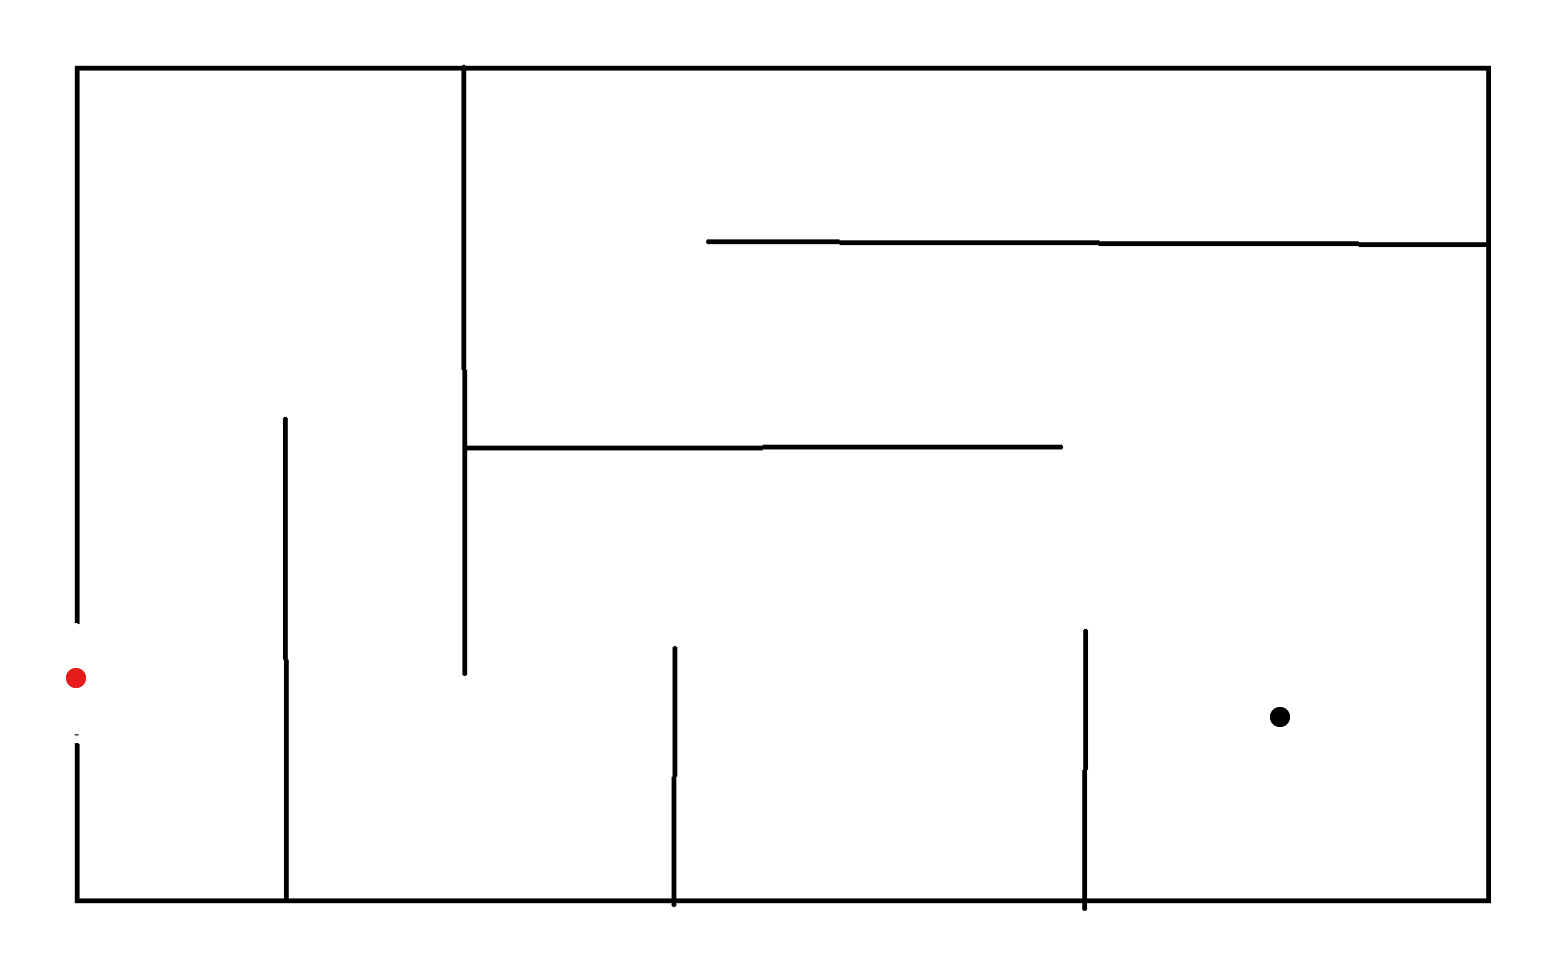
\includegraphics[width=0.5\linewidth]{demo.png}
    \caption{Hand drawn map to test go-back}
    \label{fig:placeholder}
\end{figure}
\begin{figure}
    \centering
    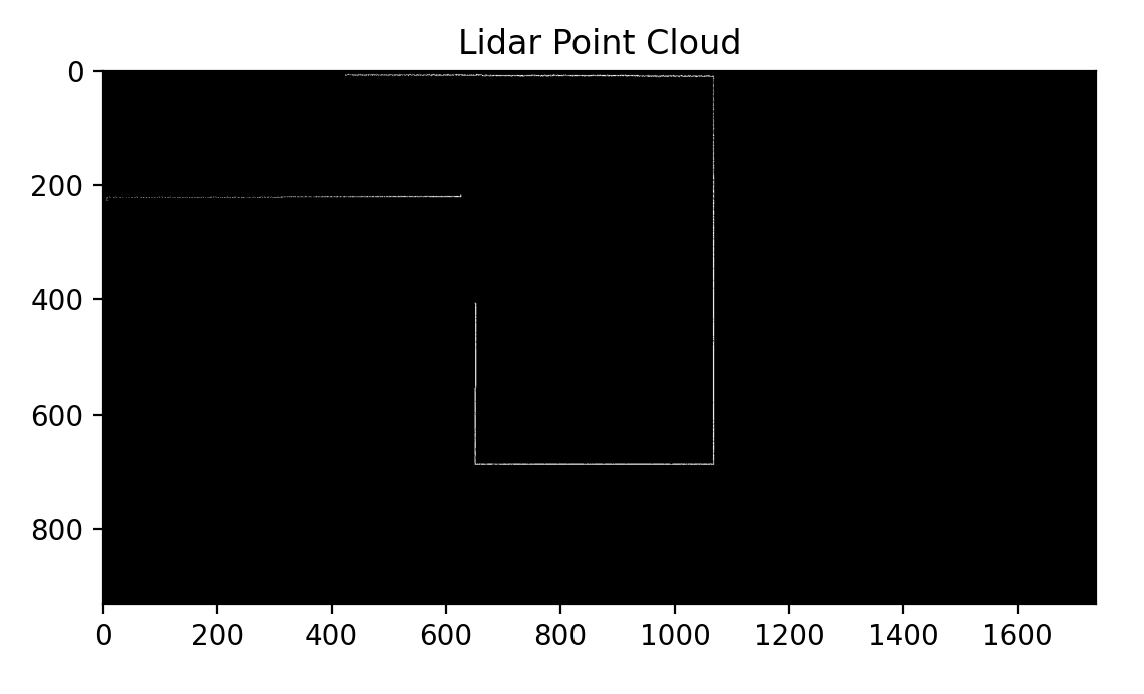
\includegraphics[width=0.5\linewidth]{lidar_cound_points.png}
    \caption{Lidar cloud points. This shows what the robot sees at that instance}
    \label{fig:placeholder}
\end{figure}
The robot is at coordinate $(1400, 750)$ (the black dot on figure $4$), and the door at the coordinate $(130, 740)$ (the red dot on figure $4$). When the code is ran, the first thing that will be displayed will be what the robot sees in that specific instance, featured in figure $5$. Then, the screen will display the possible points that it can go to, then it will choose randomly the point, such as in figure $6$. The screen will show which extremities it will add the margin to, such as in figure $7$ (the orange point). As mentioned above, to memorize the map, a green line was drawn of its path, and the blue dots are the spots it can potentially go to, including the newly generated intermediate nodes, just like in figure $8$. \\
\begin{figure}
    \centering
    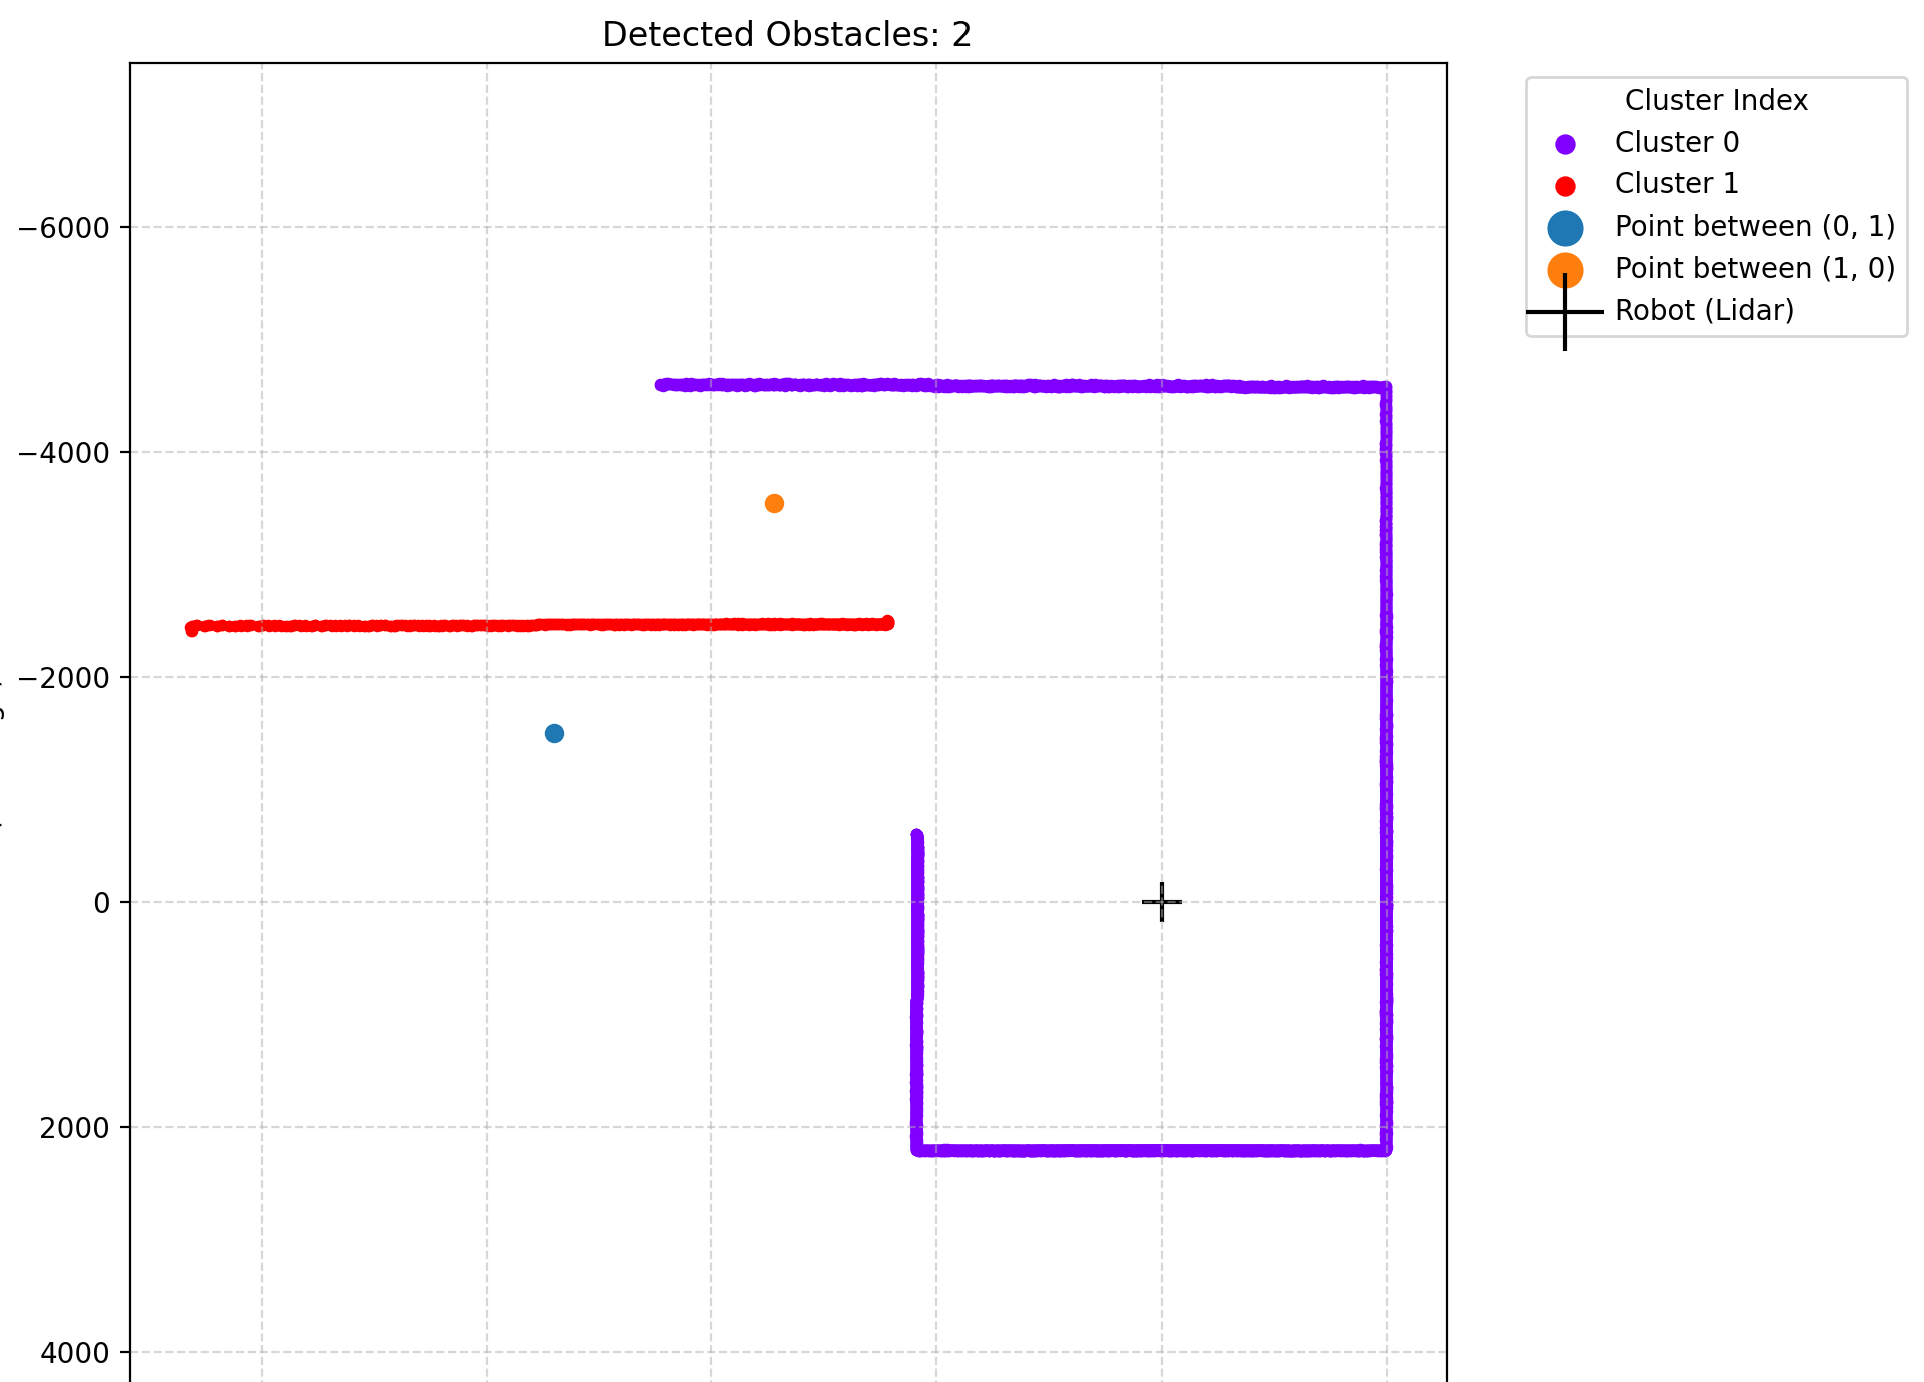
\includegraphics[width=0.5\linewidth]{middle_point.png}
    \caption{The points generated by my algorithm}
    \label{fig:placeholder}
\end{figure}
\begin{figure}
    \centering
    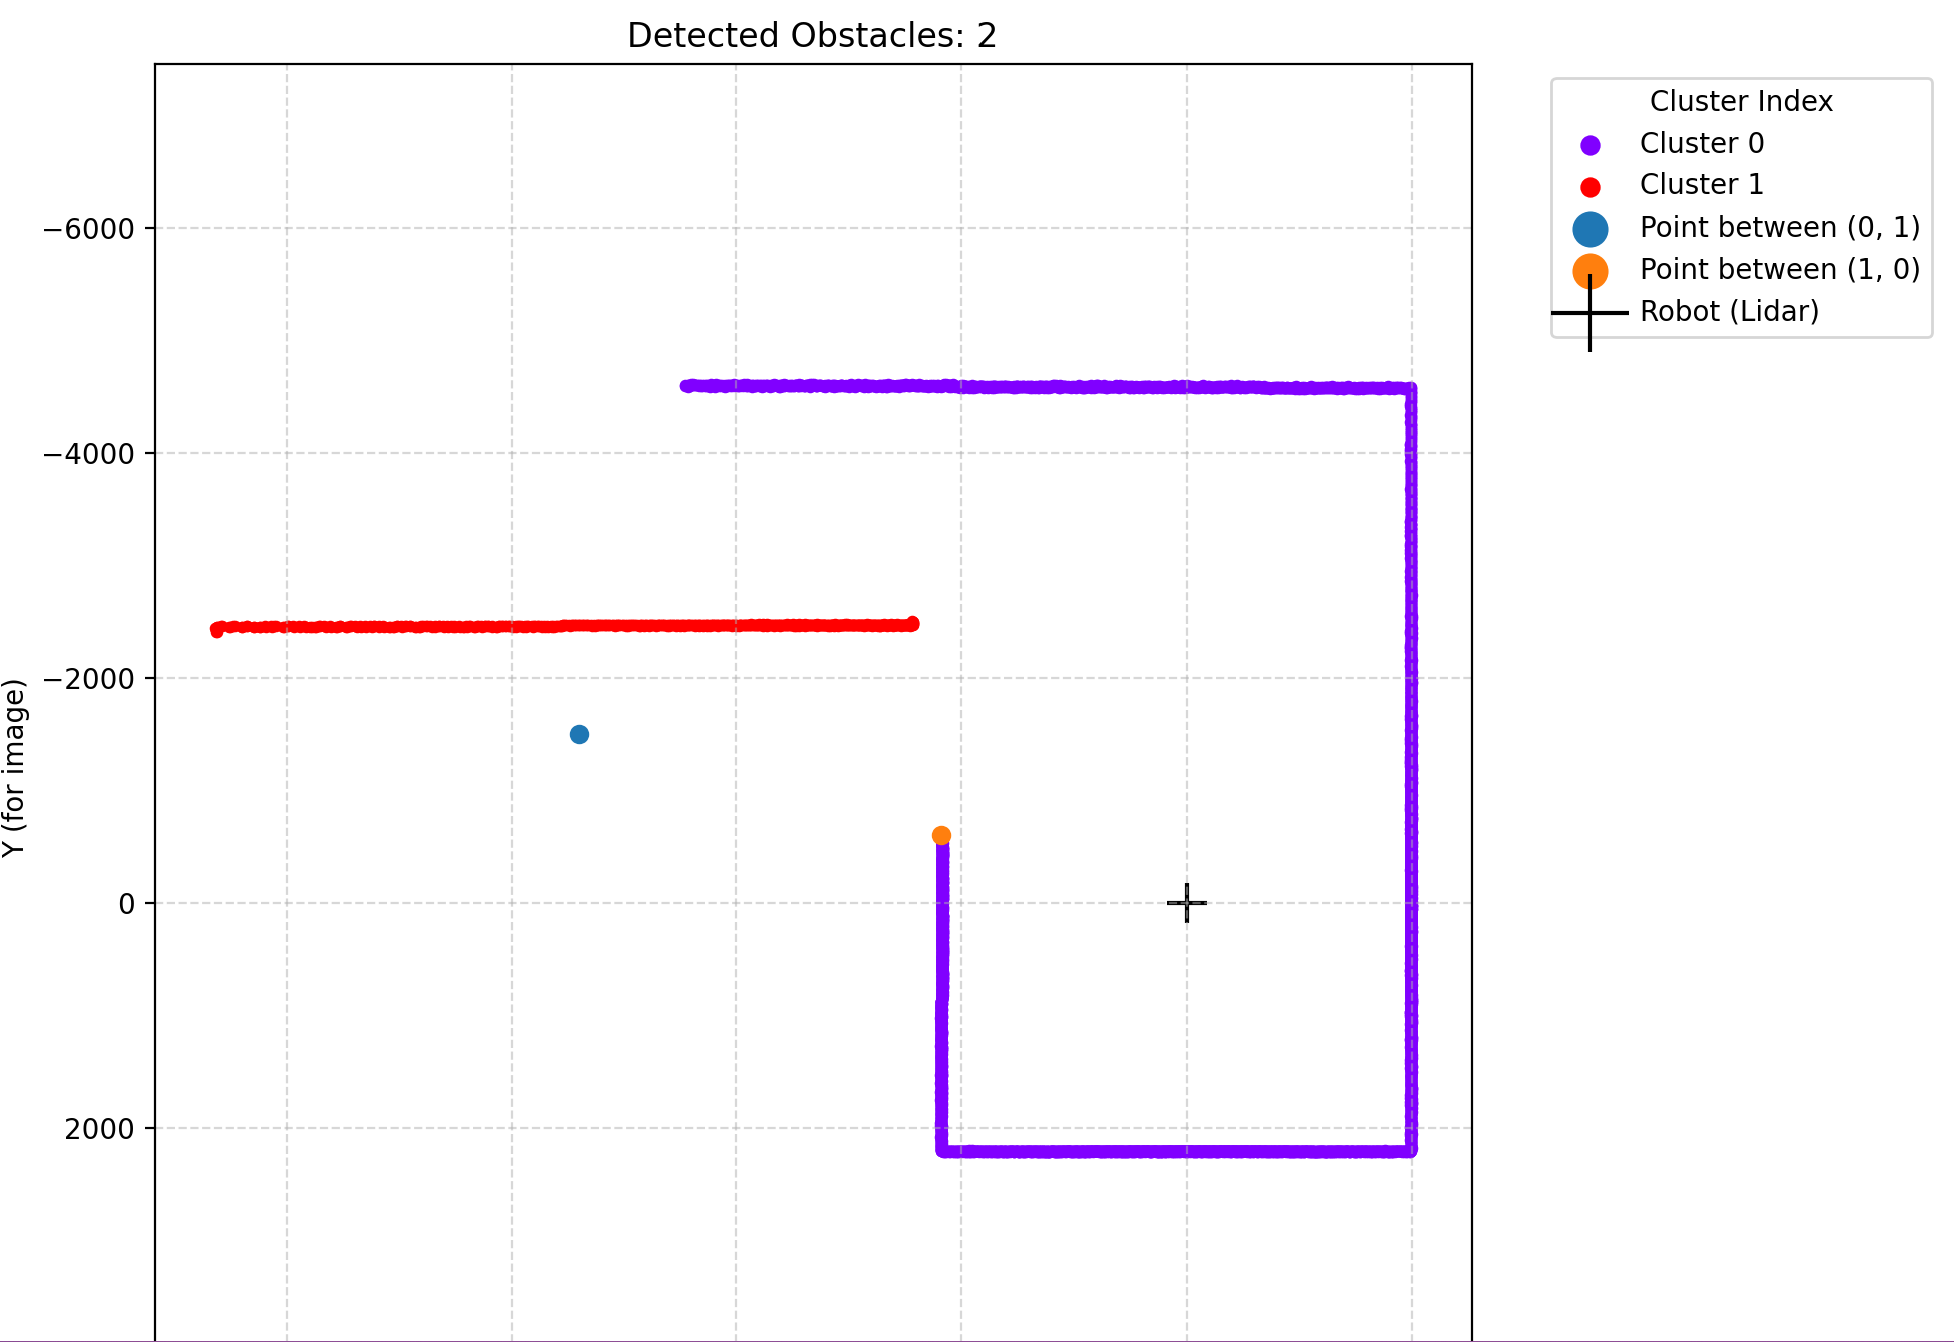
\includegraphics[width=0.5\linewidth]{extremeties.png}
    \caption{Shows which extremeties it chose and add the margin to}
    \label{fig:placeholder}
\end{figure}

In the same figure $8$, go-back is showcased to work successfully. Then, in figure $9$, the robot finally manages to find the door, and shows the overall path mapping of the robot. \\
\begin{figure}
    \centering
    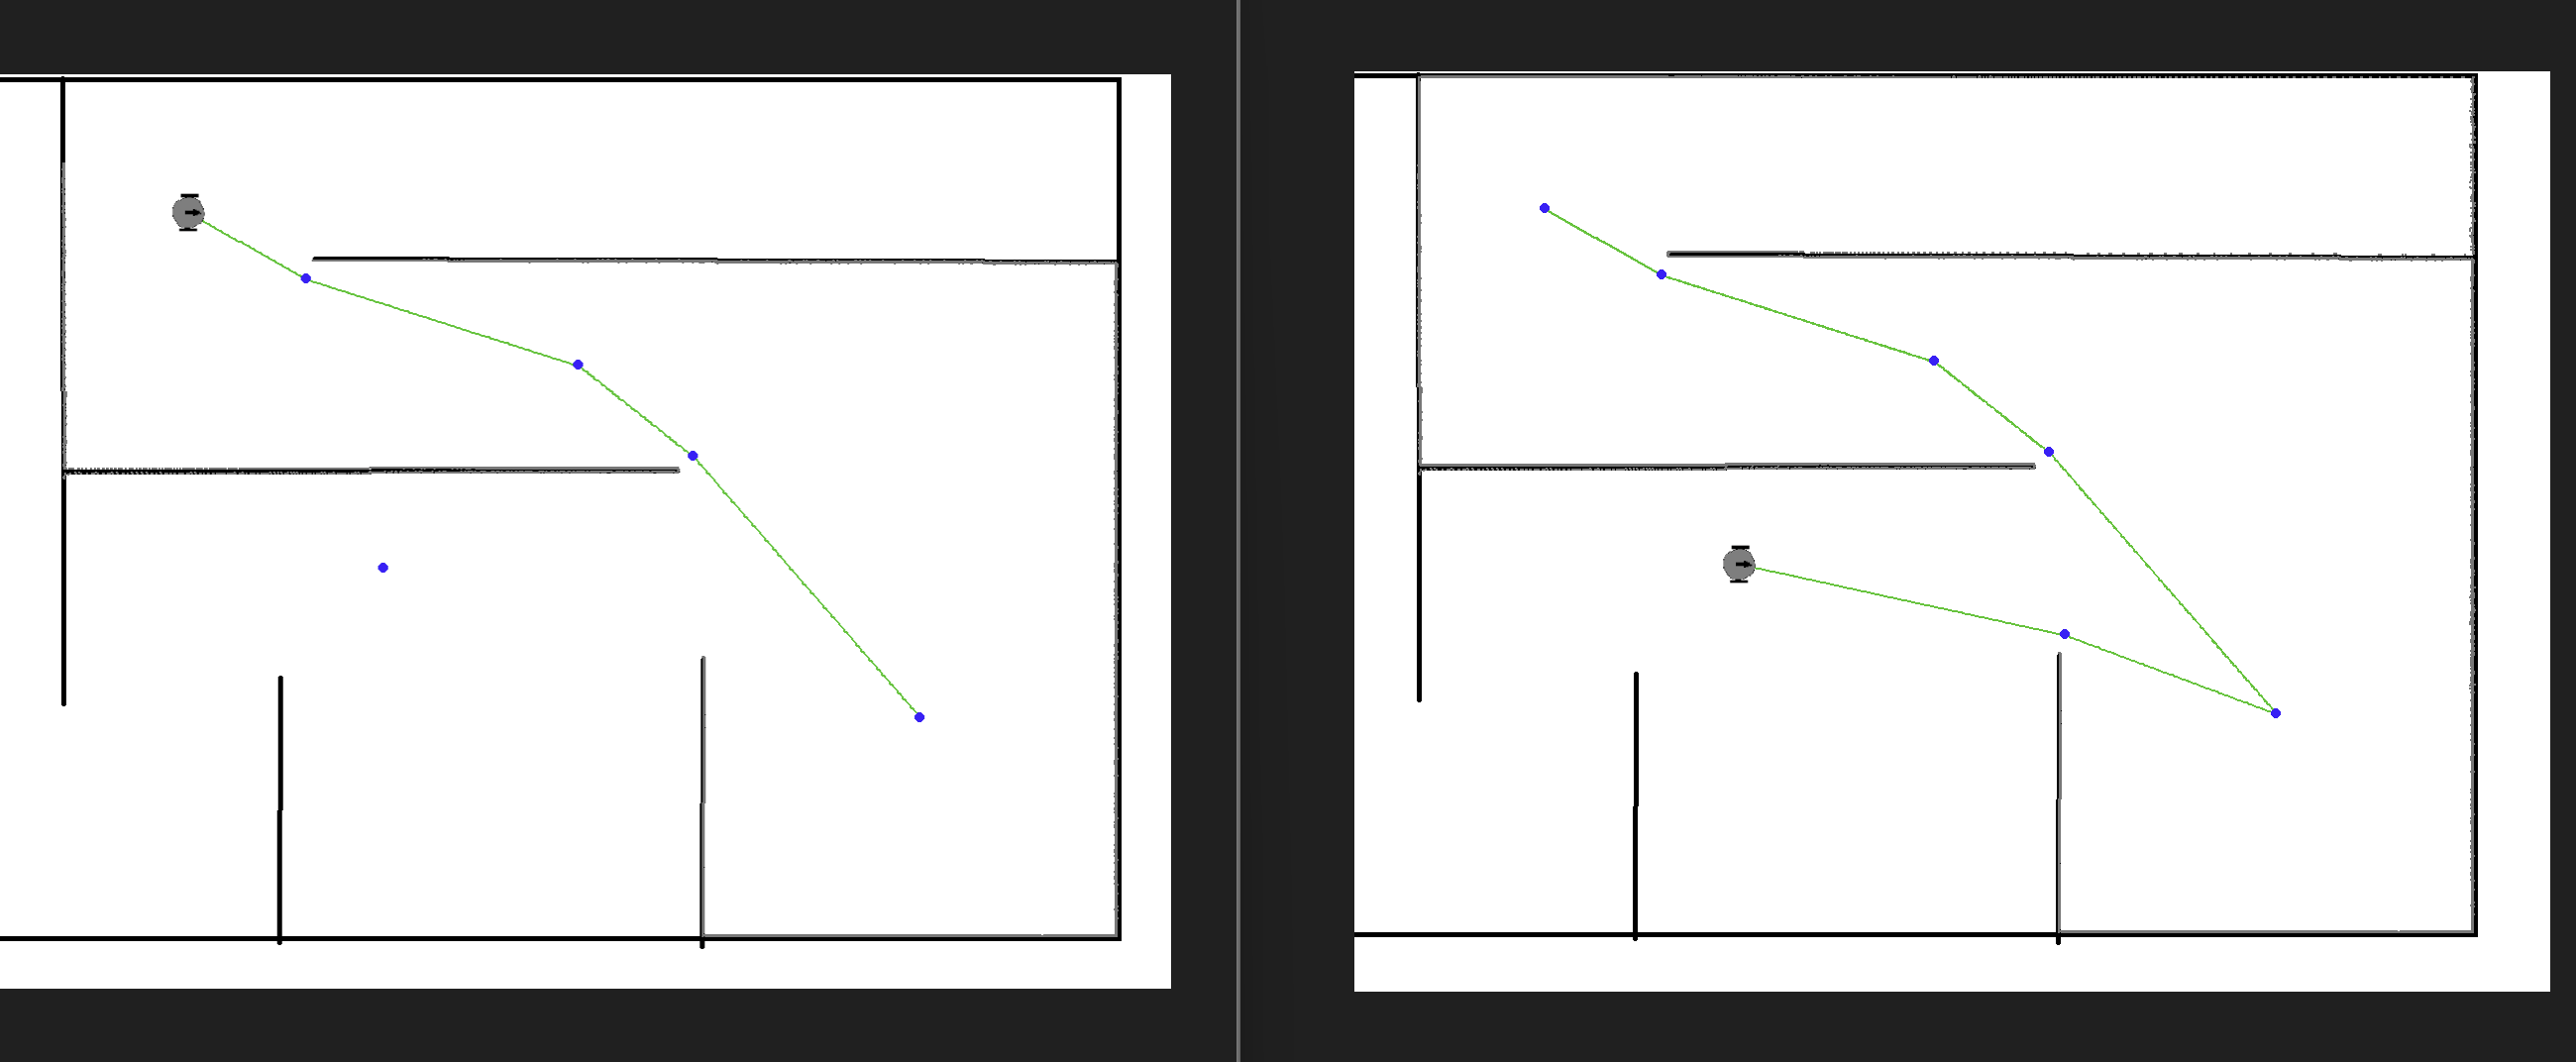
\includegraphics[width=0.5\linewidth]{go_back.png}
    \caption{Showcase how go-back works}
    \label{fig:placeholder}
\end{figure}
\begin{figure}
    \centering
    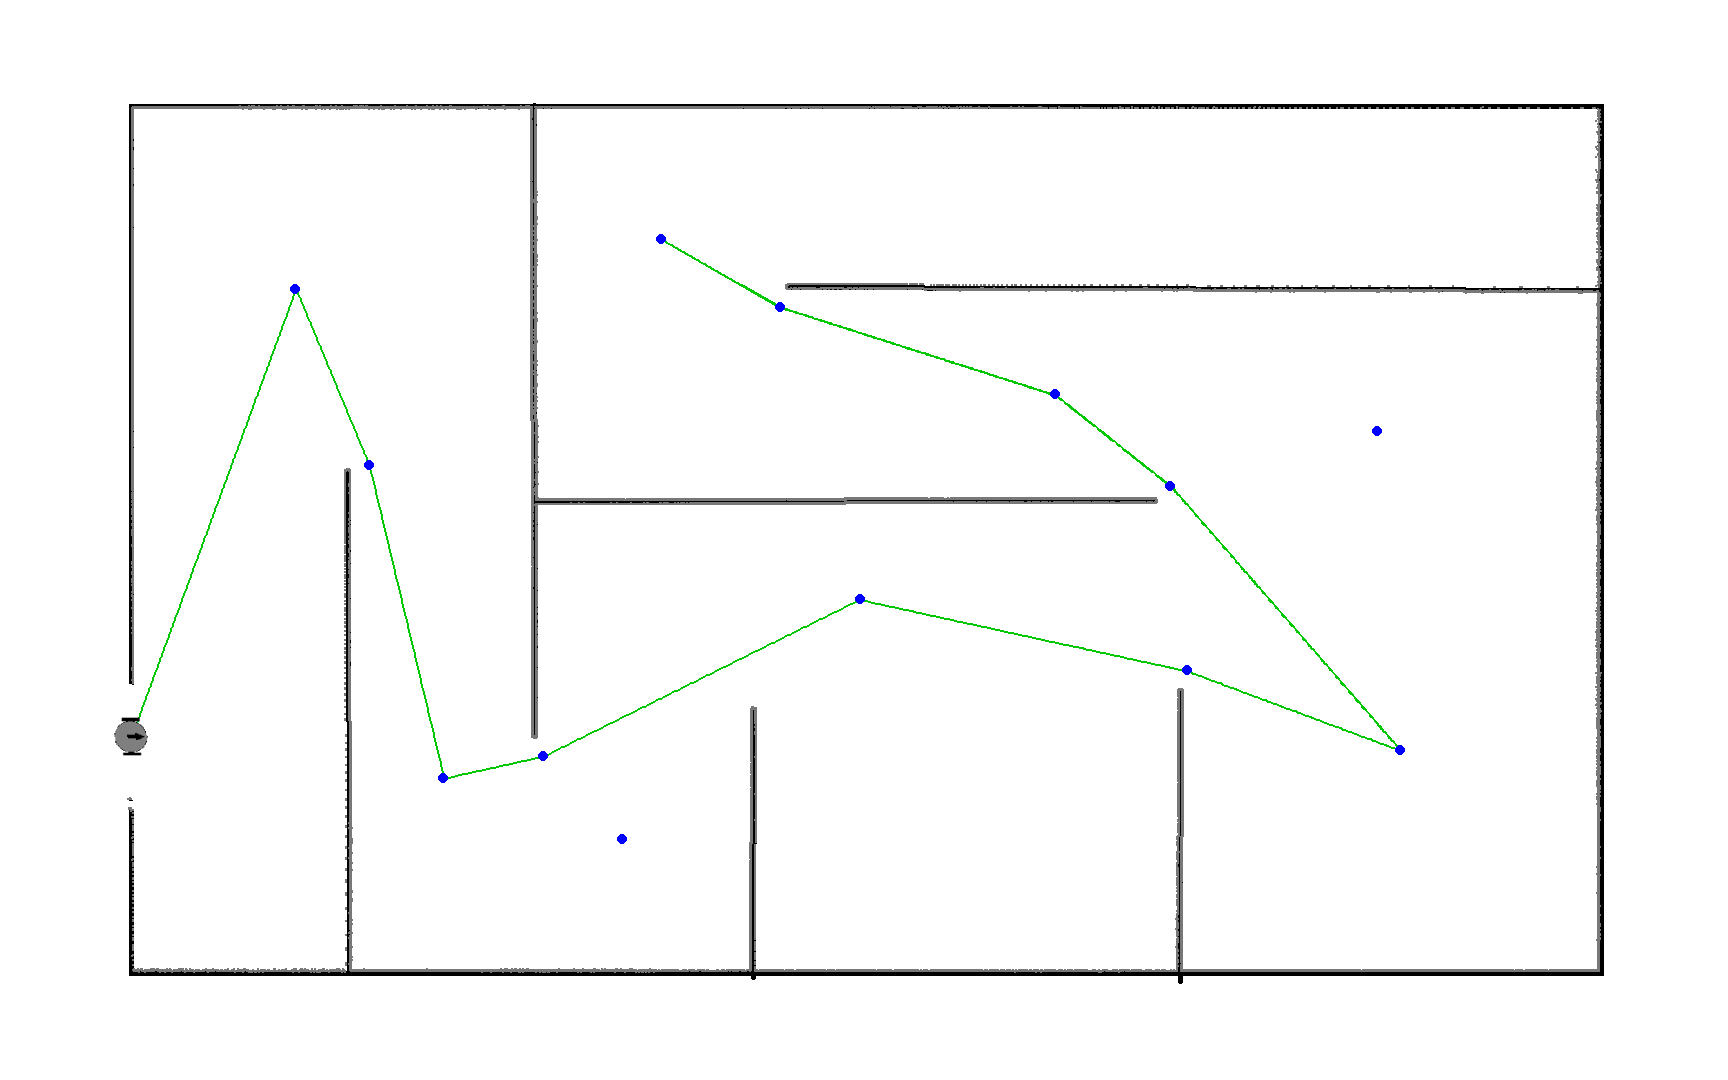
\includegraphics[width=0.5\linewidth]{final_map.png}
    \caption{The final exploration of the robot, getting successfully to the door}
    \label{fig:placeholder}
\end{figure}

As successful the algorithm is, there are a lot of improvement that needs to be done. For instance, I had a pretty big problem in my current code, that is, before heading to the intermediate node, the robot does not do a scan, hence does not see possible obstacles, therefore collides with it, such as in figure $10$. And idea would be doing a scan before going from the intermediate node to the final, but sometimes intermediate nodes could be generated inside the obstacle that is in its blind spot. Therefore it would be a future challenge to incorporate the scan checking while the robot moves, or even use the depth camera that we couldn't make it work. I have purposely left a small gap in figure $10$'s map so the robot should not go through, but since it does not see the obstacle on its right, it goes through. 

\begin{figure}
    \centering
    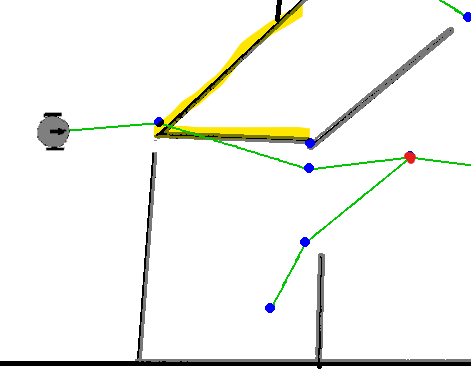
\includegraphics[width=0.5\linewidth]{blind_spot.png}
    \caption{Showcases the blind spot of the robot at a given point. The yellow highlighted obstacles can't be seen by the robot at the red point}
    \label{fig:placeholder}
\end{figure}

\newpage


\section{Conclusion}

The main part of this project lies in the development of an adaptive LiDar point clustering algorithm and a recursive obstacle avoidance path planner. Throughout the thinking and development process, I had to make a lot of pivots. While the initial plan was to look into probabilistic roadmaps and Rapidly-exploring Random trees, their reliance on an input map was not practical for our robot. It was not done in vain since it provided strong theoretical foundation. My own algorithm using the LiDAR clustering and recursive intermediate node generation offered a better and more robust solution for real-world obstacle avoidance. By including BFS, it was possible to incorporate the backtracking logic which made sure the robot recovers from dead-ends. The integration of a fine-tuned YOLO model provided the necessities for the door identification. \\

The project had a couple limitation, such as the blind spots that can't be detected before moving. Future projects and tasks could be: using a continuous SLAM integration, use a sensor fusion to prevent collisions with obstacles below or above the LiDar's view and dynamic obstacle handling to take into account the moving actors and objects. The goal is to drop as many assumptions as possible. Unfortunately with the time-frame given to me, the code has not been integrated to the main branch of the project. \\

This project showed the importance of algorithmic flexibility and the necessity of connecting the gap between high-level machine learning models and low-level sensor data parsing for successful autonomous operation.



\section{Acknowledgement}
A big thank you to professor Vybihal Joseph for supervising this project and allowing me to work on this project. I would like to thank Emile Petit that was able to help me throughout the project, especially on the new path planning algorithm, and Paul Kevorkov for helping me with the web cam. 


\printbibliography

\end{document}